%============================================================
		\section{Nombre: Disparo rojo.} \label{hab.disparoR}
		\subsubsection{Descripción}
El enemigo dispara tonalli de color rojo. El disparo de tonalli sale de enfrente del enemigo. El disparo de tonalli tendrá un desplazamiento horizontal constante. El disparo, al hacer contacto con el jugador, reducirá la cantidad de vida del jugador. Si el disparo colisiona con cualquier objeto, enemigo, ítem u obstáculo que no sea el jugador, el disparo se destruirá sin afectar el objeto, enemigo, ítem u obstáculo con el que haya colisionado. El disparo se destruirá si después de un periodo de tiempo no ha colisionado con ningún objeto o con el jugador.
		\subsubsection{Portador}
		Fantasma rojo. Ver \ref{per.fantasmaR}.
		\subsubsection{Esquema}
		Ver figura \ref{fig:disparoR}.
		\begin{figure}
			\centering
			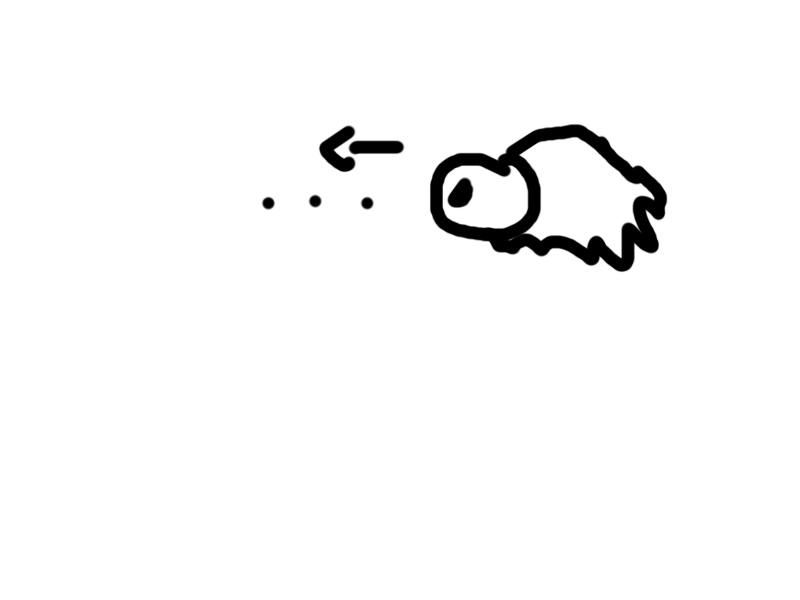
\includegraphics[height=0.2 \textheight]{Imagenes/disparoR}
			\caption{Disparo rojo.}
			\label{fig:disparoR}
		\end{figure}